\subsection{Javascript}
\label{sec:Javascript}

Die erste Version von Javascript wurde 1996 veröffentlicht. Javascript stellt eine clientseitige Skriptsprache dar, welche für dynamische Interaktion in Webbrowsern entwickelt wurde. Wie in anderen Programmiersprachen ebenfalls vorhanden, enthält Javascript eine bestimmte Anzahl von Befehlen, welche auf eine eigene Syntax aufbauen\footnotetext{\citet{powers2007}}.

Im vorliegenden Projekt wird Javascript für folgende Funktionen angewandt:

\begin{itemize}
  \item Manipulation der HTML-Struktur
  \item Anzeigen von Dialogfenstern
  \item asynchrone Serveranfragen
\end{itemize}

Die Manipulation der HTML-Struktur bedeutet, dass einzelne HTML-Elemente eines Dokuments mit Hilfe von Javascript dynamisch verändert oder gelöscht werden. Der Internetbrowser interpretiert die manipulierte HMTL-Datei neu und stellt diese dementsprechend im Browser dar.

Die Anzeige von Dialogfenstern im Browser stellt ebenfalls eine Manipulation der HTML-Struktur dar. Hierbei wird ein HTML-Element einer HTML-Datei geändert oder hinzugefügt. Dieses Element enthält einen bestimmten Text, welcher im Browser mithilfe eines Popups dargestellt wird. Mit diesem Dialogfenster kann dynamisch interagiert werden.

Javascript stellt eine rudimentäre Technologie dar, welche von Ajax genutzt wird, um asynchrone Serveranfragen zu verarbeiten. Mit Ajax können Daten gesendet und empfangen werden, ohne dass der Browser die komplette Seite neu laden muss. Es werden nur dynamisch die geänderten Werte neu geladen und aktualisiert dargestellt \footnotetext{\citet{heinle2006}}.

Die dynamische Funktionsweise von Ajax mithilfe von Javascript wird in nachfolgender Abbildung nochmal am Beispiel eines Online-Shops verdeutlicht:

\begin{figure}[htb]
\centering
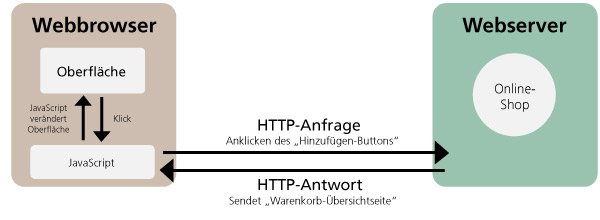
\includegraphics[width=1.0\textwidth]{GrundlagenJavascript.png}
\caption[Grundlagen Javascript]{Funktionsweise von Ajax am Beispiel\protect\footnotemark}
\label{fig:Bildergalerie}
\end{figure}
\footnotetext{Link: http://www.webmasterpro.de}

Da durch Javascript auch neue Einfallmöglichkeiten für Hacker geboten werden, ist es in allen aktuellen Browsern möglich Javascript oder bestimmte Funktionen von Javascript zu deaktivieren, um diese Sicherheitsrisiken zu reduzieren \footnotetext{\citet{steyer2010}}.